% =====================================================================
%  AGV Warehouse Automation — Software Documentation
%  Graduation Thesis (Software Subsystem)
%
%  Compile:  pdflatex AGV_Software_Documentation.tex   (run twice for TOC)
% =====================================================================
\documentclass[11pt,a4paper]{article}

\usepackage[utf8]{inputenc}
\usepackage[T1]{fontenc}
\usepackage{lmodern}
\usepackage[margin=2.4cm]{geometry}
\usepackage{amsmath,amssymb}
\usepackage{graphicx}
\usepackage{booktabs}
\usepackage{array}
\usepackage{xcolor}
\usepackage{caption}
\usepackage{enumitem}
\usepackage{fancyhdr}
\usepackage{longtable}
\usepackage{listings}
\usepackage{algorithm}
\usepackage{algpseudocode}
\usepackage{tikz}
\usetikzlibrary{positioning,arrows.meta,calc,shapes.geometric,fit,backgrounds}
\usepackage[hidelinks]{hyperref}

% ---- Colors ----------------------------------------------------------
\definecolor{accent}{HTML}{1F4E79}
\definecolor{accent2}{HTML}{2E75B6}
\definecolor{codebg}{HTML}{F5F7FA}
\definecolor{codekw}{HTML}{0F5FA6}
\definecolor{codecmt}{HTML}{6A8759}
\definecolor{codestr}{HTML}{A31515}
\definecolor{boxblue}{HTML}{DCE6F2}
\definecolor{boxgreen}{HTML}{D6E8D5}
\definecolor{boxgray}{HTML}{ECECEC}

% ---- Listings --------------------------------------------------------
\lstdefinestyle{py}{
  language=Python, backgroundcolor=\color{codebg}, basicstyle=\ttfamily\scriptsize,
  keywordstyle=\color{codekw}\bfseries, commentstyle=\color{codecmt}\itshape,
  stringstyle=\color{codestr}, numbers=left, numberstyle=\tiny\color{gray},
  frame=single, rulecolor=\color{gray!40}, breaklines=true, showstringspaces=false,
  columns=fullflexible, xleftmargin=14pt, framexleftmargin=14pt, tabsize=2}
\lstset{style=py}

% ---- Header / footer -------------------------------------------------
\pagestyle{fancy}\fancyhf{}
\lhead{\small\textcolor{accent}{AGV Warehouse Automation}}
\rhead{\small\textcolor{accent}{Software Subsystem}}
\cfoot{\thepage}
\renewcommand{\headrulewidth}{0.4pt}

\captionsetup{font=small,labelfont=bf}
\setlength{\parskip}{4pt}
\setlength{\parindent}{0pt}

% ---- Section styling -------------------------------------------------
\usepackage{titlesec}
\titleformat{\section}{\Large\bfseries\color{accent}}{\thesection}{0.6em}{}
\titleformat{\subsection}{\large\bfseries\color{accent2}}{\thesubsection}{0.6em}{}

\newcommand{\code}[1]{\texttt{\small #1}}

% =====================================================================
\begin{document}

% ---------------------------- TITLE ----------------------------------
\begin{titlepage}
\centering
\vspace*{2.2cm}
{\color{accent}\rule{\linewidth}{1.4pt}}\\[0.5cm]
{\Huge\bfseries Autonomous Guided Vehicle for\\[0.2cm] Warehouse Rack Transport}\\[0.4cm]
{\LARGE Software Subsystem --- Design, Implementation \\[0.15cm] and Validation}\\[0.3cm]
{\color{accent}\rule{\linewidth}{1.4pt}}\\[1.4cm]
{\large Graduation Thesis Documentation}\\[0.4cm]
{\large Robotics \& Autonomous Systems}\\[2.2cm]
\begin{minipage}{0.85\textwidth}\centering\small
\textit{This document presents the architecture, algorithms and iterative
engineering of the navigation, autonomous rack-docking, perception and
human--machine-interface software of a mecanum-drive AGV built on ROS~2
Jazzy, Nav2, SLAM Toolbox and Gazebo.}
\end{minipage}
\vfill
{\large \today}
\end{titlepage}

% --------------------------- ABSTRACT --------------------------------
\section*{Abstract}
\addcontentsline{toc}{section}{Abstract}
This thesis documents the software of an Autonomous Guided Vehicle (AGV)
designed to transport storage racks between locations in a simulated
warehouse. The vehicle is a four-wheel \emph{mecanum} (holonomic) platform
equipped with two planar LiDAR scanners and a vertical lift mechanism,
running the Robot Operating System~2 (ROS~2, \emph{Jazzy} distribution) with
the Nav2 navigation stack, SLAM~Toolbox localization and a custom mission
controller. The central engineering contribution is the redesign of the
rack pickup/transport/drop behaviour from a fragile \emph{open-loop} routine
into a robust \emph{closed-loop, sensor-driven} pipeline: a LiDAR leg-servo
docking controller, holonomic map- and odometry-referenced motion
primitives, a self-calibrating carried-payload perception filter, and a
web-based mission-control interface. We present the mathematical formulation
of the perception and control laws, the system architecture, and---in
chronological order---the diagnostic methodology through which each failure
mode was identified and eliminated. The final system performs a complete
autonomous transport cycle reliably in simulation and is structured to
transfer to physical hardware.

\vspace{0.4cm}
\tableofcontents
\newpage

% =====================================================================
\section{Introduction}
% =====================================================================
\subsection{Background and Motivation}
Modern warehouses increasingly rely on fleets of AGVs that slide underneath
mobile storage racks, lift them, and relocate them between storage cells and
picking stations. Unlike free-roaming delivery robots, a rack-transport AGV
must (i)~travel only along designated aisles, (ii)~dock underneath a rack
with centimetre precision so the lift engages correctly, and (iii)~manage the
fact that, while carrying a rack, the payload's legs occupy the very plane
its safety scanners observe. These constraints make the docking and
perception software substantially more demanding than ordinary point-to-point
navigation.

\subsection{Problem Statement}
The initial implementation suffered from four recurring, defect-level
failures observed during simulation testing:
\begin{enumerate}[leftmargin=1.4em,itemsep=1pt]
  \item the robot \emph{failed to centre} reliably underneath a rack;
  \item it \emph{``feared'' approaching} the rack, stalling at the aisle mouth;
  \item it \emph{failed to fully extract} a rack or to place it precisely at
        the drop-off, frequently abandoning it in the aisle;
  \item while carrying a rack the navigation stack registered the carried
        legs as \emph{ghost obstacles}, eventually trapping the vehicle.
\end{enumerate}
Each symptom is traced to a concrete root cause in
Section~\ref{sec:chrono}.

\subsection{Objectives}
\begin{itemize}[leftmargin=1.4em,itemsep=1pt]
  \item Replace all open-loop dead-reckoning motion with closed-loop,
        feedback-controlled primitives that tolerate wheel slip and
        localization drift.
  \item Achieve repeatable sub-3\,cm docking accuracy using only the
        on-board LiDAR.
  \item Allow the vehicle to ignore its own carried payload without becoming
        blind to genuine obstacles.
  \item Deliver an operator interface for mission dispatch, live monitoring
        and one-click system launch.
\end{itemize}

\subsection{Contributions}
The software contributions documented herein are: a prior-guided LiDAR
rack-pose estimator based on rigid Procrustes alignment
(Section~\ref{sec:estim}); a holonomic leg-servo docking controller with an
alignment-gated velocity law and an anti-stiction breakaway mechanism
(Section~\ref{sec:control}); a self-calibrating carried-payload scan filter
(Section~\ref{sec:filter}); and a real-time browser-based mission-control GUI
with interpolated state visualization (Section~\ref{sec:gui}).

\subsection{Document Organization}
Section~\ref{sec:arch} describes the system architecture. Sections~\ref{sec:nav}
and~\ref{sec:mission} cover the navigation/mapping and mission-management
subsystems. Sections~\ref{sec:dock}--\ref{sec:filter} present the docking and
perception methodology. Section~\ref{sec:chrono} narrates the chronological
development and validation. Section~\ref{sec:gui} documents the GUI.
Sections~\ref{sec:config}--\ref{sec:concl} give configuration, results and
conclusions.

% =====================================================================
\section{System Architecture}\label{sec:arch}
% =====================================================================
\subsection{Technology Stack}
The software runs on ROS~2 Jazzy (Ubuntu~24.04). Physics and sensing are
simulated in Gazebo (\code{gz-sim}) with a mecanum-drive plugin and an
odometry publisher; the same ROS interfaces are presented by the physical
robot, so the application software is simulator-agnostic. Autonomous
navigation uses the Nav2 stack (MPPI controller, NavFn planner, layered
costmaps, velocity smoother, collision monitor). Localization uses SLAM
Toolbox in \emph{localization} mode against a pre-built map, fused with
wheel odometry and IMU through an Extended Kalman Filter
(\code{robot\_localization}). The operator interface is a single-page
React/Vite web application communicating over \code{rosbridge}.

\subsection{Package Organization}
The workspace is divided into five ROS~2 packages
(Table~\ref{tab:packages}), separating description, bring-up, mapping,
navigation and mission control.

\begin{table}[h]\centering\small
\caption{ROS~2 package responsibilities.}\label{tab:packages}
\begin{tabular}{@{}lp{11.2cm}@{}}
\toprule
\textbf{Package} & \textbf{Responsibility}\\
\midrule
\code{agv\_description}   & URDF/Xacro robot model, mecanum-drive and lift
 plugins, meshes, Gazebo worlds, TF tree.\\
\code{agv\_bringup}       & Top-level launch of simulation world and robot
 spawn; teleoperation utilities.\\
\code{agv\_mapping}       & Dual-LiDAR scan merger and the carried-payload
 self-filter feeding SLAM and the costmaps.\\
\code{agv\_navigation}    & Nav2 parameters, EKF, laser filters, SLAM
 configuration and navigation launch files.\\
\code{agv\_mission\_control} & Mission-manager node, task/lane logic, the web
 GUI and the system launcher service.\\
\bottomrule
\end{tabular}
\end{table}

\subsection{Computational Graph}
Figure~\ref{fig:arch} shows the principal nodes and data flow. Sensor scans
are range-filtered, optionally payload-filtered, then consumed by both the
costmaps and (after merging) the localizer. The mission manager orchestrates
Nav2 through the \code{NavigateToPose} action and issues direct velocity
commands during closed-loop docking.

\begin{figure}[h]\centering
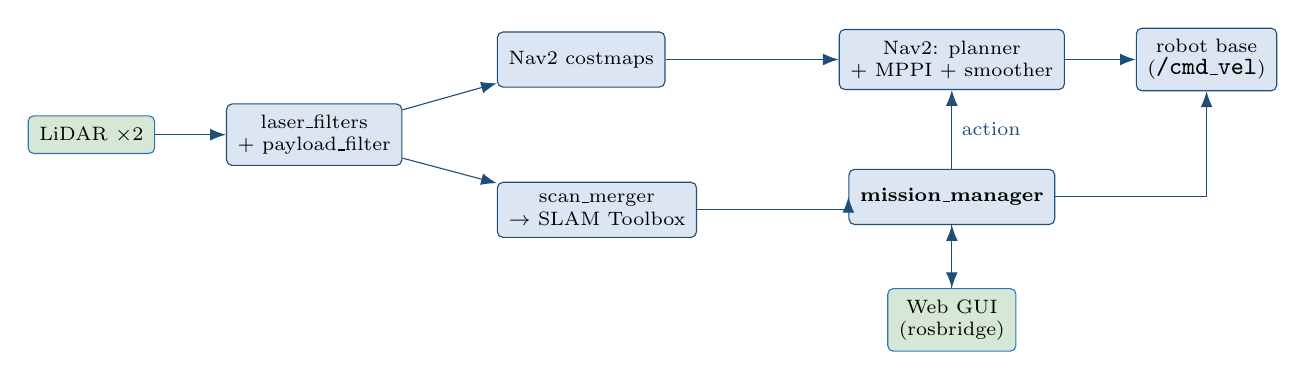
\begin{tikzpicture}[
  font=\scriptsize,
  node distance=6mm and 9mm,
  box/.style={draw=accent,fill=boxblue,rounded corners=2pt,inner sep=4pt,minimum height=7mm,align=center},
  sens/.style={draw=accent2,fill=boxgreen,rounded corners=2pt,inner sep=4pt,align=center},
  arr/.style={-{Latex[length=2mm]},accent}]
\node[sens](lidar){LiDAR $\times2$};
\node[box,right=of lidar](filt){laser\_filters\\+ payload\_filter};
\node[box,above right=2mm and 12mm of filt](cost){Nav2 costmaps};
\node[box,below right=2mm and 12mm of filt](merge){scan\_merger\\$\rightarrow$ SLAM Toolbox};
\node[box,right=22mm of cost](nav){Nav2: planner\\+ MPPI + smoother};
\node[box,below=10mm of nav](mm){\textbf{mission\_manager}};
\node[box,right=of nav](base){robot base\\(\code{/cmd\_vel})};
\node[sens,below=8mm of mm](gui){Web GUI\\(rosbridge)};
\draw[arr](lidar)--(filt);
\draw[arr](filt)--(cost); \draw[arr](filt)--(merge);
\draw[arr](cost)--(nav); \draw[arr](merge.east)-|(mm.west);
\draw[arr](nav)--(base);
\draw[arr](mm)-- node[right]{action} (nav);
\draw[arr](mm.east)-| (base.south);
\draw[arr](gui)--(mm);
\draw[arr](mm)--(gui);
\end{tikzpicture}
\caption{Simplified computational graph. Green: sensing/HMI; blue: processing.}
\label{fig:arch}
\end{figure}

\subsection{Coordinate Frames}
The TF tree follows the REP-105 convention:
\code{map}~$\rightarrow$~\code{odom}~$\rightarrow$~\code{base\_footprint}, with
sensor frames rigidly attached to the base. \code{map}~$\rightarrow$~\code{odom}
is published by SLAM Toolbox (correcting drift), while
\code{odom}~$\rightarrow$~\code{base\_footprint} is the continuous, locally
smooth EKF estimate. The docking controllers deliberately reference
different frames depending on the task: leg-servoing operates in
\code{base\_footprint}, exact placement uses \code{map}, and straight pull-out
uses \code{odom} for jump-free relative motion.

\subsection{Key Interfaces}
Table~\ref{tab:topics} lists the principal topics and the action interface.

\begin{table}[h]\centering\small
\caption{Principal ROS interfaces.}\label{tab:topics}
\begin{tabular}{@{}llp{6.8cm}@{}}
\toprule
\textbf{Name} & \textbf{Type} & \textbf{Role}\\
\midrule
\code{/scan\_front,\,/scan\_rear} & \code{LaserScan} & Raw dual LiDAR.\\
\code{/scan\_*\_nav} & \code{LaserScan} & Payload-filtered scans to costmaps/SLAM.\\
\code{/odometry/filtered} & \code{Odometry} & EKF pose/velocity.\\
\code{/cmd\_vel} & \code{Twist} & Final body velocity to the base.\\
\code{/plan} & \code{Path} & Nav2 global plan (visualised).\\
\code{/rack\_obstacles} & \code{PointCloud2} & Dynamic rack-leg obstacles.\\
\code{/payload/leg\_mask} & \code{Float32MultiArray} & Carried-leg mask (latched).\\
\code{/mission\_control/state} & \code{String\,(JSON)} & Full mission state to GUI.\\
\code{navigate\_to\_pose} & action & Goal dispatch to Nav2.\\
\bottomrule
\end{tabular}
\end{table}

% =====================================================================
\section{Navigation and Mapping Subsystem}\label{sec:nav}
% =====================================================================
\subsection{Localization and the Sensor Pipeline}
The two LiDARs are individually range-filtered, then a custom
\code{scan\_merger} node reprojects both into a common frame and emits a
unified 360$^\circ$ scan (\code{/scan\_merged}) for SLAM Toolbox. SLAM runs in
localization mode, matching live scans against a stored map and publishing
the \code{map}$\rightarrow$\code{odom} correction. Wheel odometry from the
mecanum plugin and IMU data are fused by the EKF into the smooth
\code{/odometry/filtered} estimate used as the Nav2 odometry source.

\subsection{Layered Costmaps}
The local costmap is a rolling 3\,m voxel grid; the global costmap is a static
map overlaid with an obstacle layer. Both subscribe to the payload-filtered
scans and to \code{/rack\_obstacles}, a latched point cloud the mission manager
publishes containing the four corner legs of every \emph{occupied} rack so
the planner avoids storage cells that are physically blocked. An inflation
layer pads obstacles; its radius is switched at runtime
(Section~\ref{sec:mission}).

\subsection{MPPI Controller and the Velocity Pipeline}
Trajectory tracking uses Nav2's Model-Predictive Path-Integral (MPPI)
controller configured with an \emph{omni} motion model to exploit the
holonomic base. Its critics weight goal/path alignment, forward preference,
and a footprint-aware cost critic. The output traverses a fixed pipeline
(Figure~\ref{fig:vel}); crucially the controller publishes to
\code{/cmd\_vel\_nav}, \emph{not} \code{/cmd\_vel}, so that when the mission
manager assumes direct control during docking there is no contention on the
final velocity topic---a property exploited and verified in
Section~\ref{sec:chrono}.

\begin{figure}[h]\centering
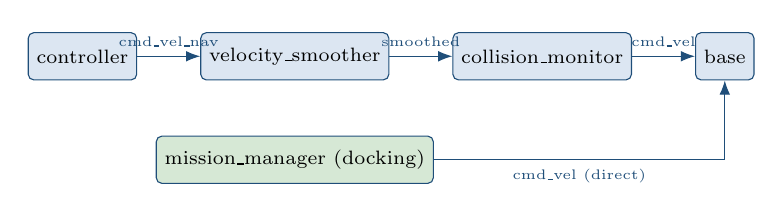
\begin{tikzpicture}[font=\scriptsize,node distance=6mm,
  b/.style={draw=accent,fill=boxblue,rounded corners=2pt,inner sep=3pt,minimum height=6mm},
  arr/.style={-{Latex[length=1.8mm]},accent}]
\node[b](c){controller};
\node[b,right=8mm of c](s){velocity\_smoother};
\node[b,right=8mm of s](cm){collision\_monitor};
\node[b,right=8mm of cm](r){base};
\node[b,below=7mm of s,fill=boxgreen](mm){mission\_manager (docking)};
\draw[arr](c)--node[above]{\tiny cmd\_vel\_nav}(s);
\draw[arr](s)--node[above]{\tiny smoothed}(cm);
\draw[arr](cm)--node[above]{\tiny cmd\_vel}(r);
\draw[arr](mm.east)-|node[pos=0.25,below]{\tiny cmd\_vel (direct)}(r.south);
\end{tikzpicture}
\caption{Velocity pipeline. The smoother caps autonomous travel speed; the
mission manager bypasses it for closed-loop docking.}\label{fig:vel}
\end{figure}

% =====================================================================
\section{Mission Management}\label{sec:mission}
% =====================================================================
The \code{mission\_manager} node is the application brain: it maintains a task
queue, sequences Nav2 goals and lift commands, performs closed-loop docking,
and streams state to the GUI.

\subsection{State Machine}
Mission execution is governed by the finite-state machine of
Figure~\ref{fig:fsm}. A transport task expands into an ordered sequence of
navigation, docking, lifting, extraction, placement and retreat phases.

\begin{figure}[h]\centering
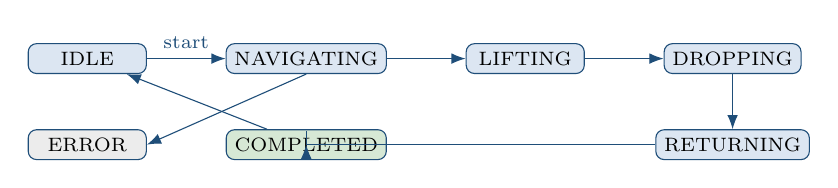
\begin{tikzpicture}[font=\scriptsize,node distance=10mm,
  s/.style={draw=accent,fill=boxblue,rounded corners=3pt,inner sep=3pt,minimum width=15mm},
  arr/.style={-{Latex[length=1.8mm]},accent}]
\node[s](idle){IDLE};
\node[s,right=of idle](nav){NAVIGATING};
\node[s,right=of nav](lift){LIFTING};
\node[s,right=of lift](drop){DROPPING};
\node[s,below=7mm of drop](ret){RETURNING};
\node[s,below=7mm of nav,fill=boxgreen](done){COMPLETED};
\node[s,below=7mm of idle,fill=boxgray](err){ERROR};
\draw[arr](idle)--node[above]{start}(nav);
\draw[arr](nav)--(lift); \draw[arr](lift)--(drop);
\draw[arr](drop)--(ret); \draw[arr](ret)-|(done);
\draw[arr](done)--(idle);
\draw[arr](nav.south)--(err.east);
\end{tikzpicture}
\caption{Mission-execution state machine (abridged).}\label{fig:fsm}
\end{figure}

\subsection{Task Model and Persistence}
Locations (racks, drop zones, dock and aisle \emph{lanes}) are persisted to a
JSON file under \code{\textasciitilde/.ros} so operator edits survive
rebuilds. Each rack/zone carries a runtime \code{state} of \code{free} or
\code{occupied}; a transport task validates that its source is occupied and
its destination free before accepting it, and atomically flips both states as
the rack is lifted and dropped.

\subsection{Lane-Graph Routing}
Operators draw aisle polylines that the manager compiles into an undirected
graph (endpoints within 0.5\,m are merged into shared nodes). Routing to a
rack proceeds by: (i)~projecting the rack onto the lane network to find the
perpendicular \emph{approach foot} on the aisle-facing side; (ii)~running
Dijkstra's algorithm from the robot's nearest lane node to the foot's
segment; and (iii)~commanding Nav2 along the resulting waypoints with the
final heading aligned to the rack's approach axis. This forces all rack
approaches to occur perpendicular to the aisle, mirroring real warehouse
traffic rules.

\subsection{Dynamic Costmap Reconfiguration}
During a transport the manager reconfigures the costmaps over the parameter
services: it lowers the inflation radius for the pickup approach, switches to
a larger \emph{carrying} footprint after lifting, and excludes the target
rack from \code{/rack\_obstacles} so the planner will permit the robot to
drive \emph{underneath} it rather than treating it as a lethal wall.

% =====================================================================
\section{Closed-Loop Rack Docking}\label{sec:dock}
% =====================================================================
\subsection{Why Open-Loop Docking Fails}
The original routine drove a fixed distance using
$t = d / v$ dead-reckoning with no feedback. On a mecanum platform---which
slips substantially in both simulation and reality---the achieved distance
never equals the commanded distance, so the robot lifted off-centre, failed
to fully extract the rack, and missed the drop coordinate. The redesign
replaces every final-approach motion with one of three closed-loop
primitives, each referenced to the most appropriate frame
(Table~\ref{tab:prims}).

\begin{table}[h]\centering\small
\caption{Closed-loop motion primitives.}\label{tab:prims}
\begin{tabular}{@{}lll p{5.2cm}@{}}
\toprule
\textbf{Primitive} & \textbf{Feedback} & \textbf{Frame} & \textbf{Use}\\
\midrule
\code{dock\_servo} & LiDAR legs & base & Pickup centering (x, y, yaw).\\
\code{drive\_to\_map\_point} & localization & map & Exact drop placement.\\
\code{drive\_straight} & odometry & odom & Extraction / retreat (no swing).\\
\bottomrule
\end{tabular}
\end{table}

\subsection{Rack-Pose Estimation}\label{sec:estim}
Let the robot pose in the map be $(x_r,y_r,\theta_r)$ and the stored rack pose
$(x_m,y_m,\theta_m)$. The \emph{prior} rack centre and axis expressed in the
robot's \code{base\_footprint} frame are
\begin{equation}
\begin{bmatrix}\hat c_x\\ \hat c_y\end{bmatrix}=
R(-\theta_r)\begin{bmatrix}x_m-x_r\\ y_m-y_r\end{bmatrix},
\qquad \hat\psi=\mathrm{wrap}(\theta_m-\theta_r),
\end{equation}
where $R(\cdot)$ is the 2-D rotation matrix and $\mathrm{wrap}$ maps to
$(-\pi,\pi]$. From these, four predicted leg positions
$\mathbf p_i$ are generated at the rack corners $(\pm a,\pm a)$,
$a=\mathrm{rack\_side}/2$, rotated by $\hat\psi$ and offset by
$(\hat c_x,\hat c_y)$.

Each raw LiDAR return is transformed into the base frame using the live
sensor TF and clustered (single-pass nearest-centroid, 12\,cm radius); only
clusters within a search window of the predicted centre are retained, which
rejects clutter from adjacent racks. Each predicted leg is then greedily
matched to its nearest observed cluster $\mathbf o_i$ within a gate.

Given $n\!\ge\!2$ correspondences, the rigid transform $(\delta\theta,\mathbf t)$
that best maps prediction to observation, minimising
$\sum_i\lVert\mathbf o_i-(R(\delta\theta)\mathbf p_i+\mathbf t)\rVert^2$, is the
closed-form 2-D Procrustes (Umeyama) solution:
\begin{equation}
\delta\theta=\operatorname{atan2}\!\Big(\textstyle\sum_i \tilde p_{i,x}\tilde o_{i,y}-\tilde p_{i,y}\tilde o_{i,x},\;
\sum_i \tilde p_{i,x}\tilde o_{i,x}+\tilde p_{i,y}\tilde o_{i,y}\Big),
\quad \mathbf t=\bar{\mathbf o}-R(\delta\theta)\bar{\mathbf p},
\end{equation}
where $\tilde{(\cdot)}$ denotes centroid-subtracted points and
$\bar{(\cdot)}$ the centroids. Applying this correction to the prior yields
the refined rack pose in the base frame,
$(c_x,c_y,c_\psi)$, which is what the controller servos on. Because the
estimate is anchored to the \emph{observed} legs, it is robust to
localization drift: the controller converges on the true rack regardless of
map error.

\subsection{Leg-Servo Control Law}\label{sec:control}
With the rack pose error in the base frame defined as
$e_x=c_x,\; e_y=c_y,\; e_\psi=c_\psi$ (we drive the robot centre onto the rack
centre and align headings), the holonomic command is
\begin{align}
\omega &= \mathrm{sat}(k_\psi e_\psi,\;\omega_{\max}),\qquad
v_y = \mathrm{sat}(k_y e_y,\;v_{y,\max}),\\[2pt]
g &= \mathrm{clip}\!\Big(1-\tfrac{(|e_y|-\tau)^+}{g_y}-\tfrac{(|e_\psi|-\tau_\psi)^+}{g_\psi},\;
 g_{\min},\;1\Big),\\[2pt]
v_x &= g\cdot \mathrm{sat}(k_x e_x,\;v_{x,\max}),
\end{align}
where $(\cdot)^+=\max(0,\cdot)$ and $\mathrm{sat},\mathrm{clip}$ are
saturation operators. The \emph{alignment gate} $g$ throttles forward motion
when the robot is laterally or rotationally misaligned, so it squares up
before committing to drive deep between the legs; the floor $g_{\min}$
guarantees the robot always creeps inward (preventing a deadlock far from the
rack where leg geometry is poorly observed). Convergence is declared when
$|e_x|,|e_y|<\tau$ and $|e_\psi|<\tau_\psi$ hold for $N$ consecutive cycles.
Algorithm~\ref{alg:dock} summarises the loop.

\begin{algorithm}[h]
\caption{Leg-servo docking (15\,Hz)}\label{alg:dock}
\begin{algorithmic}[1]
\State $\text{conv}\gets0,\ \text{lost}\gets0$
\While{not converged and not timed-out}
  \State $E \gets \textsc{EstimateRackInBase}(x_m,y_m,\theta_m)$
  \If{$E=\varnothing$}
     \State $\text{lost}\mathrel{+}=1$;\ \textbf{stop};\ \textbf{if} $\text{lost}>L$ \textbf{then} \Return \textsc{DriveToMapPoint}
  \Else
     \State $(e_x,e_y,e_\psi)\gets E$;\ \text{lost}$\gets0$
     \If{$|e_x|,|e_y|<\tau \wedge |e_\psi|<\tau_\psi$}
        \State $\text{conv}\mathrel{+}=1$;\ \textbf{if} $\text{conv}\ge N$ \textbf{then} \Return success
     \Else\ $\text{conv}\gets0$ \EndIf
     \State compute $(v_x,v_y,\omega)$ via Eqs.~(3)--(5)
     \State $(v_x,v_y)\gets\textsc{Breakaway}(v_x,v_y)$ \Comment{anti-stiction}
     \State publish $(v_x,v_y,\omega)$
  \EndIf
\EndWhile
\end{algorithmic}
\end{algorithm}

\subsection{Anti-Stiction Breakaway}
A persistent failure was a momentary mechanical catch as the wheels passed
between the near legs: the platform stalled despite a non-zero command. The
breakaway monitors the measured EKF velocity and declares a stall when the
robot is dragging below a fraction $\rho$ of the commanded speed; after a
short debounce it boosts the command to a high breakaway velocity along the
commanded direction until motion resumes. Formally, with commanded
$\mathbf v_c$ and measured $\mathbf v_m$, a stall holds while
$\lVert\mathbf v_c\rVert>\varepsilon \wedge \lVert\mathbf v_m\rVert<\rho\lVert\mathbf v_c\rVert$;
if sustained for $T$, the output is rescaled to magnitude $v_\text{break}$.
The ratio formulation (rather than ``velocity near zero'') was essential, as
the catch produces a partial drag, not a full stop.

\subsection{Drive Primitives}
\code{drive\_straight\_closed\_loop} integrates the \code{odom} TF to drive a
signed distance along the heading while a proportional term holds lateral
offset and yaw at zero---this keeps a carried rack from swinging into its
neighbours during extraction. \code{drive\_to\_map\_point} is a holonomic
proportional servo onto an absolute map coordinate, used for exact drop
placement where there are no legs to observe.

% =====================================================================
\section{Carried-Payload Perception Filter}\label{sec:filter}
% =====================================================================
\subsection{The Self-Occlusion Problem}
A latent-lift AGV raises a rack only a few centimetres, so the four legs
remain in the LiDAR plane throughout transport, rigidly fixed in the robot
frame. Left untreated they are marked as obstacles; because they occlude the
space behind them they leave an un-clearable trail that progressively cages
the vehicle and, via SLAM, contaminates the map with ghost obstacles that
later fail navigation. Raising the lift to clear the scanner is a
simulation-only artifice that does not transfer to hardware.

\subsection{Self-Calibrating Box Mask}
The adopted solution exploits the one invariant: once lifted, the legs are
\emph{static in the base frame}. At dock convergence the manager snapshots
the \emph{measured} leg coordinates and publishes them as a latched mask. A
lightweight \code{payload\_filter} node transforms every incoming scan return
into the base frame and deletes any point falling inside the carried-rack
bounding box (the four legs plus a small margin), passing everything else
through unchanged; it is a pure pass-through when not carrying. Masking the
\emph{measured} box rather than a nominal guess makes it robust to real-world
placement variance, and because nothing physical can exist underneath a
carried rack, the masked region is provably free.
Figure~\ref{fig:filter} shows the integration: both the costmaps and the SLAM
merger consume the filtered streams, so neither the live obstacle layer nor
the map is ever contaminated.

\begin{figure}[h]\centering
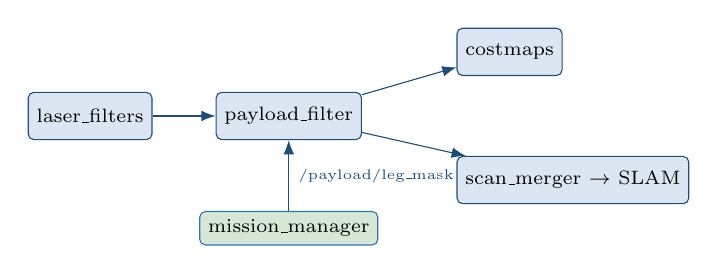
\begin{tikzpicture}[font=\scriptsize,node distance=6mm,
  b/.style={draw=accent,fill=boxblue,rounded corners=2pt,inner sep=3pt,minimum height=6mm,align=center},
  g/.style={draw=accent2,fill=boxgreen,rounded corners=2pt,inner sep=3pt,align=center},
  arr/.style={-{Latex[length=1.8mm]},accent}]
\node[b](f){laser\_filters};
\node[b,right=8mm of f](p){payload\_filter};
\node[b,above right=2mm and 12mm of p](cm){costmaps};
\node[b,below right=2mm and 12mm of p](sl){scan\_merger $\to$ SLAM};
\node[g,below=9mm of p](mm){mission\_manager};
\draw[arr](f)--(p);
\draw[arr](p)--(cm); \draw[arr](p)--(sl);
\draw[arr](mm)--node[right]{\tiny /payload/leg\_mask}(p);
\end{tikzpicture}
\caption{Carried-payload filter feeding both perception consumers.}
\label{fig:filter}
\end{figure}

% =====================================================================
\section{Chronological Development and Validation}\label{sec:chrono}
% =====================================================================
The system was developed and hardened through an evidence-driven debugging
loop: each simulation run produced telemetry that localised a single root
cause, which was fixed and re-tested. Table~\ref{tab:chrono} records this
history in order; the narrative below highlights the most instructive
diagnoses.

\begin{longtable}{@{}p{0.5cm}p{5.2cm}p{8.6cm}@{}}
\caption{Chronological defect-diagnosis log.}\label{tab:chrono}\\
\toprule
\textbf{\#} & \textbf{Observed symptom} & \textbf{Root cause $\rightarrow$ resolution}\\
\midrule
\endfirsthead
\toprule
\textbf{\#} & \textbf{Observed symptom} & \textbf{Root cause $\rightarrow$ resolution}\\
\midrule
\endhead
1 & Robot ``fears'' the rack mouth & Pickup staging at 0.55\,m placed the
 footprint over the near legs $\rightarrow$ moved staging fully outside the
 footprint; the precise drive is delegated to \code{dock\_servo}.\\
2 & Target rack treated as a wall & Source rack stayed in \code{/rack\_obstacles}
 during approach $\rightarrow$ suppressed the active docking target.\\
3 & Inexact extraction/drop & Open-loop timed crawl $\rightarrow$ replaced by the
 three closed-loop primitives (Sec.~\ref{sec:dock}).\\
4 & Servo never converged & Alignment gate hit zero at Nav2's residual error
 $\rightarrow$ added gate floor; loosened tolerances to LiDAR-realistic levels.\\
5 & Robot at $\sim$10\% of commanded speed & Hypothesised topic contention;
 instrumentation of \code{cmd\_vel} vs \code{/odometry/filtered} proved the
 pipeline clean and the \emph{wheels faithful}---isolating the cause to a
 mechanical catch.\\
6 & 5\,s stall at the rack entrance & Stiction catch $\rightarrow$ ratio-based
 breakaway (Sec.~\ref{sec:control}).\\
7 & Carried legs caged the robot & Legs in the scanner plane $\rightarrow$
 self-calibrating box mask (Sec.~\ref{sec:filter}).\\
8 & Return-to-dock failed (ghost map) & Only the costmap was filtered; SLAM
 still saw legs $\rightarrow$ routed the SLAM merger through the filtered scans.\\
9 & Rack dragged on retreat & No settle delay $\rightarrow$ added a post-drop
 dwell before reversing.\\
10 & Fixes ``not taking effect'' & A YAML parameter file silently overrode the
 code defaults $\rightarrow$ made the YAML the single source of truth.\\
\bottomrule
\end{longtable}

\textbf{Diagnosis \#5 (velocity instrumentation).} The most subtle
investigation concerned a robot moving at a tenth of its commanded speed.
Rather than guess, we enumerated the publishers on \code{/cmd\_vel}, proved
the Nav2 smoother/collision chain idle during docking, and added a live
telemetry line reporting commanded versus EKF-measured velocity. The data
showed measured velocity tracking commanded velocity \emph{exactly} once
moving---definitively exonerating wheel traction and redirecting effort to
the true mechanical catch (\#6). This illustrates the project's central
methodological principle: \emph{measure, do not assume}.

\textbf{Diagnosis \#10 (configuration precedence).} Several controller
improvements appeared ineffective because a launched parameter file
overrode the in-code defaults; the staging distance, in particular, remained
at the original 0.55\,m. Recognising that YAML parameters supersede declared
defaults resolved a class of ``phantom'' regressions and motivated
consolidating all tunables in one configuration file.

% =====================================================================
\section{Web-Based Mission Control GUI}\label{sec:gui}
% =====================================================================
\subsection{Architecture}
The operator interface is a React (Vite) single-page application that
connects to \code{rosbridge} over WebSocket. It subscribes to the JSON
mission state, the feedback log and the Nav2 global plan, and publishes
operator commands. A small companion HTTP \emph{launcher} service---running
independently of ROS so it is reachable even when the stack is down---lets
the operator start the simulation or real-robot system and stop it cleanly,
directly from the header.

\subsection{Smooth Live Map}
The map is rendered on an HTML canvas driven by a \code{requestAnimationFrame}
loop decoupled from React. Because the mission state arrives at only 5\,Hz, a
naive redraw makes the robot icon step and lag; instead the displayed pose is
exponentially interpolated toward each update,
$\mathbf p \leftarrow \mathbf p + (1-e^{-k\,\Delta t})(\mathbf p^\star-\mathbf p)$,
yielding fluid 60\,fps motion with a fading trail. The canvas renders a metric
grid, the operator-drawn lanes, the live Nav2 plan, the dock, and every
rack/zone coloured strictly by its \code{free}/\code{occupied} state. The true
robot footprint and heading are drawn, and the carried rack is outlined while
lifting.

\subsection{Defects Resolved}
Three latent GUI defects were corrected: (i)~drawn lanes vanished because the
state-merge silently dropped the \code{lanes} field on every update;
(ii)~rack colours never changed after a transport because the task payload
omitted the location \code{id} the backend keys its state updates on; and
(iii)~the speed slider had no effect on autonomous travel because it scaled
only teleoperation---it now drives the Nav2 velocity-smoother limit. The live
global-plan overlay was added to mirror the path visualisation familiar from
RViz.

% =====================================================================
\section{Configuration and Parameters}\label{sec:config}
% =====================================================================
All docking, drive and timing parameters are exposed as ROS parameters in a
single YAML file so the system can be tuned without recompilation and
re-tuned on hardware. Table~\ref{tab:params} lists the principal values.

\begin{table}[h]\centering\small
\caption{Selected mission-manager parameters (final tuned values).}\label{tab:params}
\begin{tabular}{@{}llp{6.6cm}@{}}
\toprule
\textbf{Parameter} & \textbf{Value} & \textbf{Meaning}\\
\midrule
\code{pickup\_approach\_distance} & 1.35\,m & Aisle staging point, outside the rack footprint.\\
\code{inflation\_radius\_pickup}  & 0.25\,m & Low, so MPPI is not repelled by the legs on approach.\\
\code{dock\_vx\_max / vy\_max}     & 0.28 / 0.18\,m/s & Docking speed caps.\\
\code{dock\_pos\_/yaw\_tolerance}  & 0.03\,m / 0.05\,rad & Convergence thresholds.\\
\code{dock\_vx\_floor}            & 0.30 & Minimum forward gate (anti-deadlock).\\
\code{breakaway\_velocity}        & 0.55\,m/s & Anti-stiction punch-through.\\
\code{stall\_ratio / stall\_time} & 0.40 / 0.35\,s & Stall detection.\\
\code{extract\_/retreat\_clearance} & 1.15\,m & Straight pull-out distance.\\
\code{drop\_wait\_time}           & 5.0\,s & Settle dwell before reversing.\\
\code{box\_margin} (filter)       & 0.12\,m & Payload mask margin.\\
\bottomrule
\end{tabular}
\end{table}

% =====================================================================
\section{Results and Discussion}\label{sec:results}
% =====================================================================
After the development cycle of Section~\ref{sec:chrono}, the AGV performs a
complete autonomous transport---aisle routing, perpendicular approach,
LiDAR-servo docking, lift, straight extraction, transit, exact placement and
retreat, followed by return-to-dock---reliably in simulation. Reported
docking residuals settle to approximately $(0.03,\,0.00)$\,m with sub-degree
yaw error using only on-board LiDAR, validating the Procrustes-based
estimator and the gated control law. The carried-payload filter eliminated
both the self-caging and the ghost-map failure, and the breakaway removed the
need for manual intervention at the rack entrance.

Two limitations remain. First, the docking momentum and breakaway thresholds
were tuned against the simulated mecanum friction model and will require
re-tuning on hardware---though, by design, every primitive is closed-loop and
the parameters are externalised for exactly this purpose. Second, the box
mask blanks the rack-footprint region around the robot while carrying; this
is safe in wide aisles but its margin must be kept modest in very tight
spaces so that near-field obstacles just beyond the rack remain visible.

% =====================================================================
\section{Conclusion and Future Work}\label{sec:concl}
% =====================================================================
This work transformed an unreliable, open-loop rack-handling routine into a
robust closed-loop system founded on three principles: \emph{servo on what
you can sense} (LiDAR legs rather than dead-reckoning), \emph{reference each
motion to the most appropriate frame}, and \emph{measure before you fix}. The
resulting architecture---a prior-guided rigid-alignment pose estimator, an
alignment-gated holonomic controller with anti-stiction recovery, a
self-calibrating payload filter, and a real-time operator GUI---delivers
repeatable autonomous transport and is structured for hardware transfer.

Future work includes: on-robot re-tuning and a friction-identification
procedure; replacing the box mask with an oriented per-leg mask for tighter
aisles; multi-AGV fleet coordination over the lane graph; and a learned
estimator to extend leg detection to partially occluded or non-square racks.

% =====================================================================
\appendix
\section{Build and Run}
\begin{lstlisting}[language={},numbers=none,basicstyle=\ttfamily\scriptsize]
# Build the workspace
colcon build --symlink-install && source install/setup.bash

# One-shot launch (simulation)
ros2 launch agv_navigation navigation_sim.launch.py mode:=2_lidars
ros2 launch agv_mission_control mission_control.launch.py

# Or use the GUI launch buttons via the launcher service:
python3 src/agv_mission_control/launcher_server.py        # always-on
cd src/agv_mission_control/gui && npm run dev -- --host    # serve GUI
\end{lstlisting}

\end{document}
